\documentclass{beamer}
\usepackage{beamerthemesplit}
\usepackage{subfig}
\usepackage{amssymb,amsmath,mathtools}
\usepackage{amsfonts,booktabs}
\usepackage{lmodern,textcomp}
\usepackage{color}
\usepackage{tikz}
\usepackage{natbib}
\usepackage{multicol}
\usepackage{ctex}
\usepackage[level]{datetime}
\usepackage{listings}


\usetheme{Warsaw}
\newdateformat{ukdate}{\monthname[\THEMONTH] \ordinaldate{\THEDAY} , \THEYEAR}
\lstset{
 columns=fixed,       
 numbers=left,                                        % 在左侧显示行号
 numberstyle=\tiny\color{gray},                       % 设定行号格式
 frame=none,                                          % 不显示背景边框
 backgroundcolor=\color[RGB]{245,245,244},            % 设定背景颜色
 keywordstyle=\color[RGB]{40,40,255},                 % 设定关键字颜色
 numberstyle=\footnotesize\color{darkgray},           
 commentstyle=\it\color[RGB]{0,96,96},                % 设置代码注释的格式
 stringstyle=\rmfamily\slshape\color[RGB]{128,0,0},   % 设置字符串格式
 showstringspaces=false,                              % 不显示字符串中的空格
 language=c++,                                        % 设置语言
}


\title{基于生成式先验的人像视频编辑}
\author{汪兆辰}
\date{\ukdate\today}

\begin{document}

\begin{frame}
    \titlepage
\end{frame}

\section{前端页面}

\begin{frame}
    \frametitle{前端页面}
    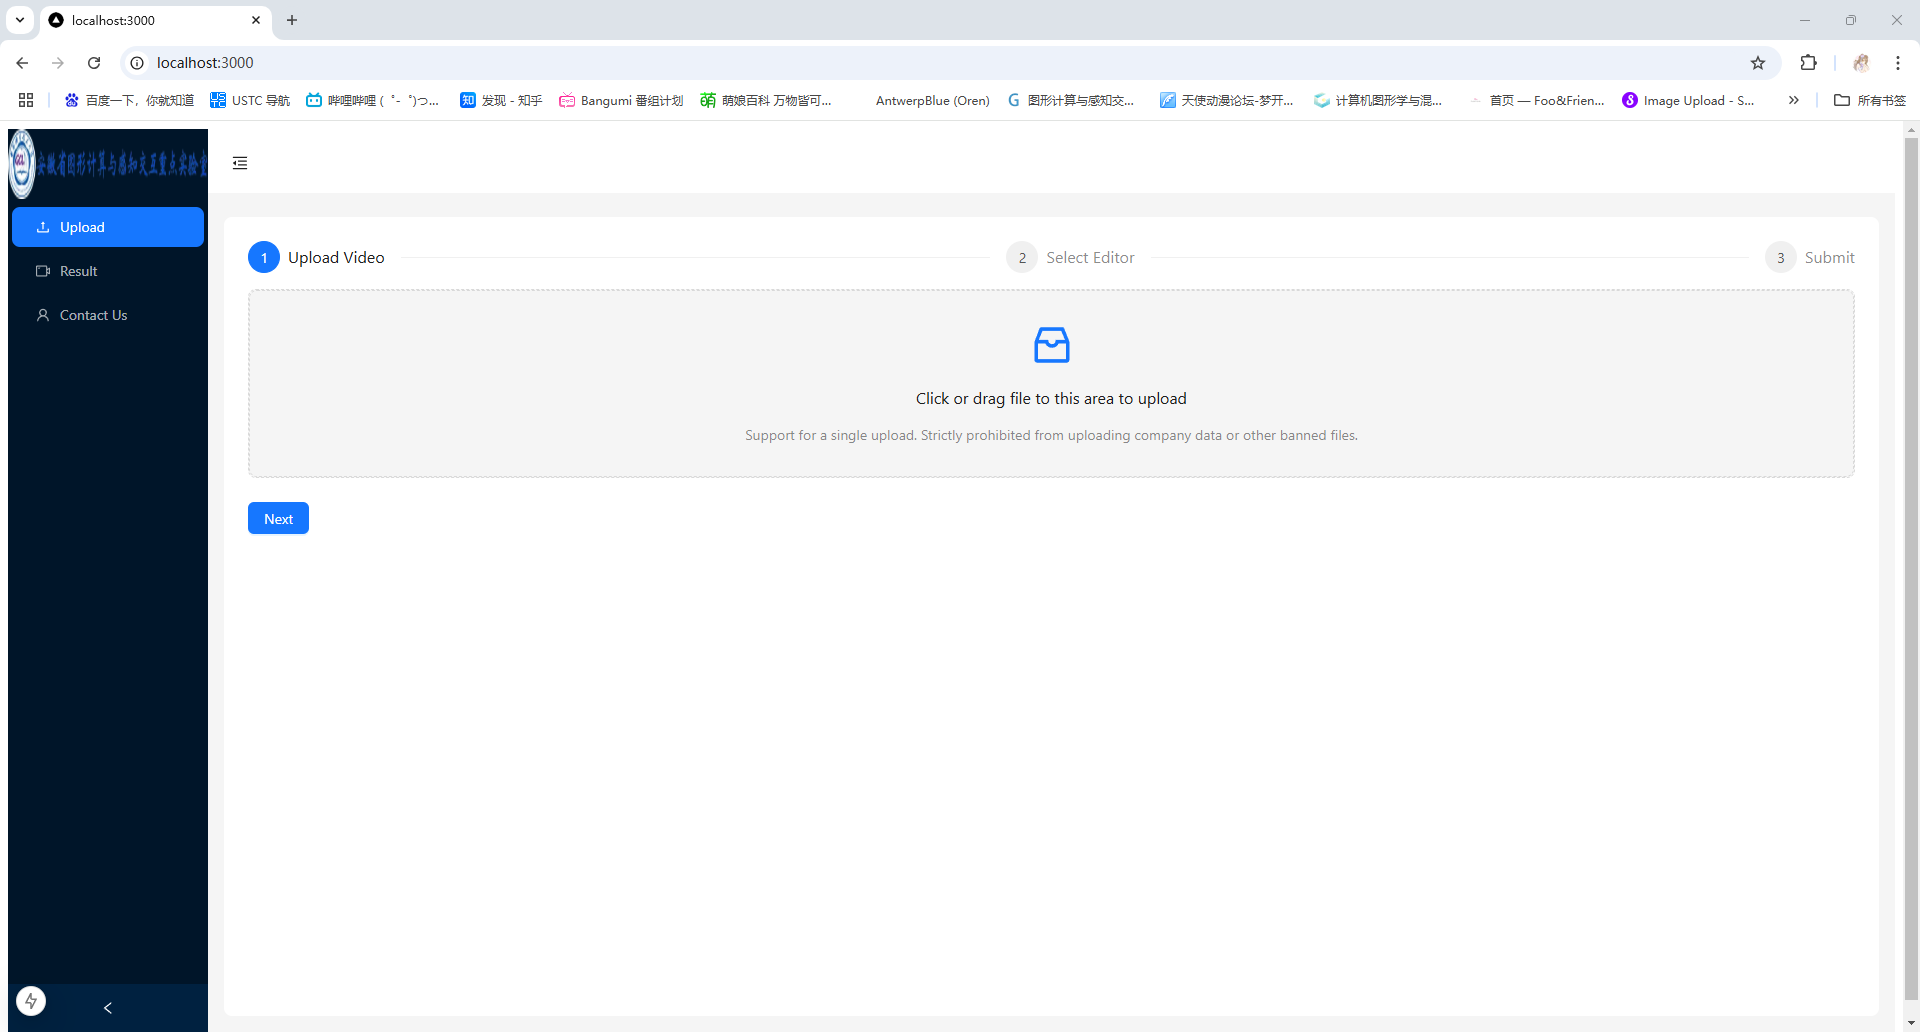
\includegraphics[width=\textwidth]{pic2.png}
\end{frame}


\section{后端业务}

\begin{frame}
    \frametitle{后端架构}
    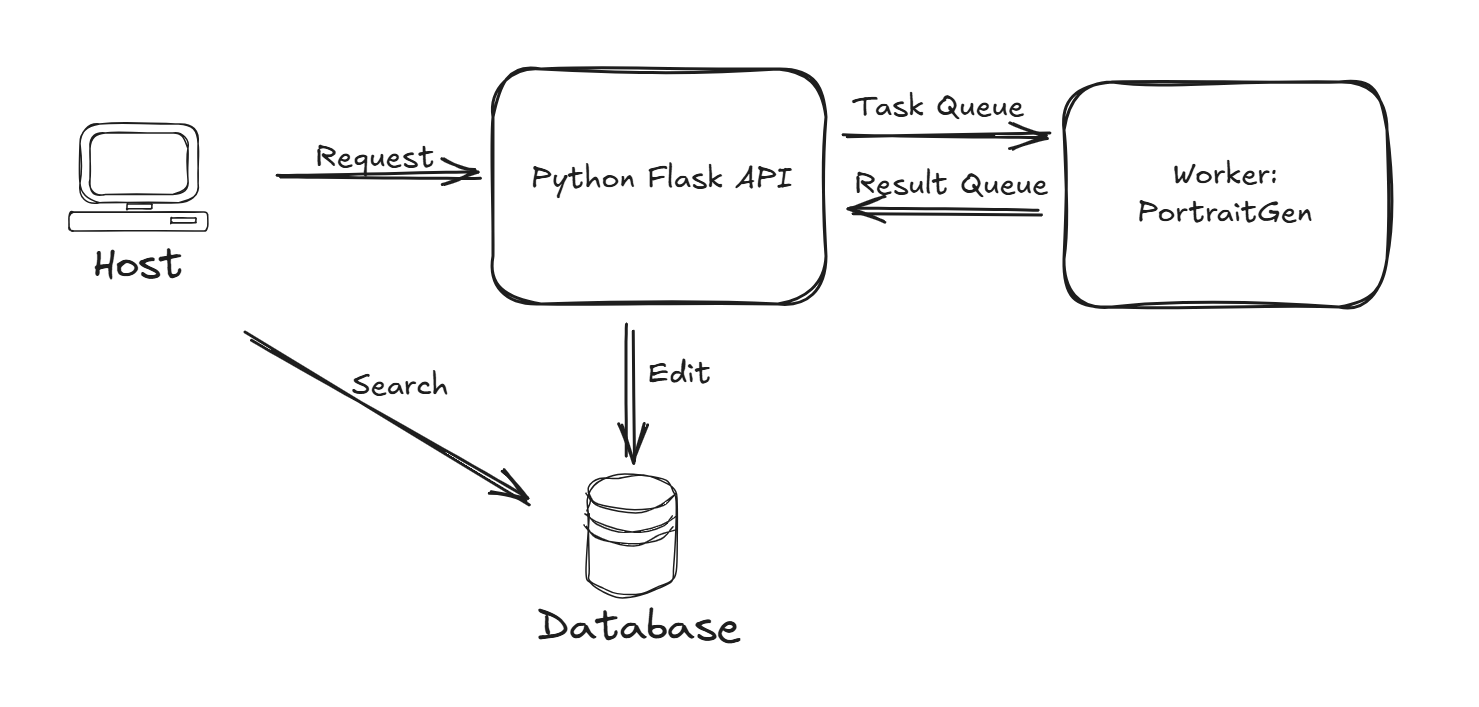
\includegraphics[width=0.9\textwidth]{pic1.png}
    \begin{itemize}
        \item 前端采用Next.js框架搭建页面,后端使用Python的Flask框架搭建API,数据库采用MySQL与Redis
        \item 前端实现用户的视频与Prompt上传,向API发送请求后通过Redis构建任务队列管理并发,在处理完毕后发回前端
    \end{itemize}

\end{frame}

\begin{frame}
    \frametitle{数据库设计}
    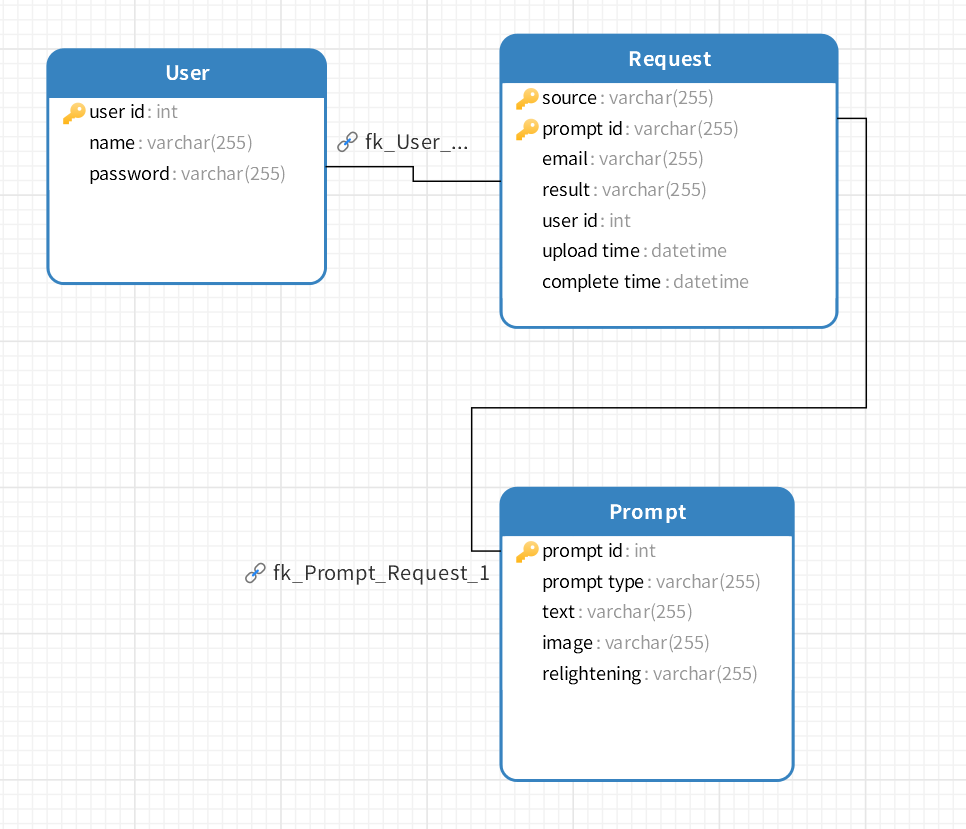
\includegraphics[width=0.8\textwidth]{pic3.png}
\end{frame}

\begin{frame}
    \frametitle{目前进展}
    \begin{itemize}
        \item 前端页面与后端API基本完成,后续需要添加任务队列管理功能与连接数据库
        \item 需要添加用户验证功能以支持结果的访问与查找,同时避免未授权用户大量上传任务导致服务器压力过大
        \item 前端页面的Result栏实际上是数据库的查找,需要在连接数据库后实现
        \item 代码目前部署在本地开发环境,在开发完成后需要部署到服务器上
        \item 前端在开发时比较粗糙,在正式上线前需要美化
    \end{itemize}

\end{frame}

\begin{frame}
    
\includegraphics[width=0.9\textwidth]{pic4.png}
    \begin{itemize}
        \item 语音驱动的可交互二次元形象已经有比较成熟的应用,利用gpt-sovits可以生成角色语音,也有Lipsync等语音驱动模型
    \end{itemize}
\end{frame}

\end{document}